\documentclass[a4paper,10pt]{report}
\usepackage[utf8]{inputenc}
\usepackage[T1]{fontenc}
\usepackage[frenchb]{babel}
\frenchbsetup{StandardLists=true}
\usepackage{enumitem}
\usepackage{lmodern} % Pour changer le pack de police
\usepackage{makeidx}
\usepackage{circuitikz}
%\usepackage{amsmath}
%\usepackage{amssymb}
%\usepackage{mathrsfs}
\usepackage{graphicx}
\usepackage{url}
\usepackage{array}
\newcolumntype{M}[1]{>{\raggedright}m{#1}}
\title{Rapport travail 1 \\EZMeal}
\author{Groupe R\\ \\Jean-Benoît Berlier\\Laurent Desausoi \\ Martin Fockedey \\Maxime Mawait \\Arthur Van Stratum 
}
\date{\today}
\makeindex

\begin{document}
\begin{titlepage}
\begin{figure}[t]

\includegraphics[scale=0.3]{epl-logo.jpg}
\end{figure}

\maketitle 
\end{titlepage}

\tableofcontents

\pagebreak

\chapter{Avant-propos}

Dans le cadre du cours de conception orientee objet, il nous a ete demande de realiser une application de cuisine pour une chaine de supermarches: "EZMeal".
Ce document reprend les differents choix de conception effectue lors de la conception du schema ORM et des bases de donnees liees.

\begin{figure}[!h]
	\center
	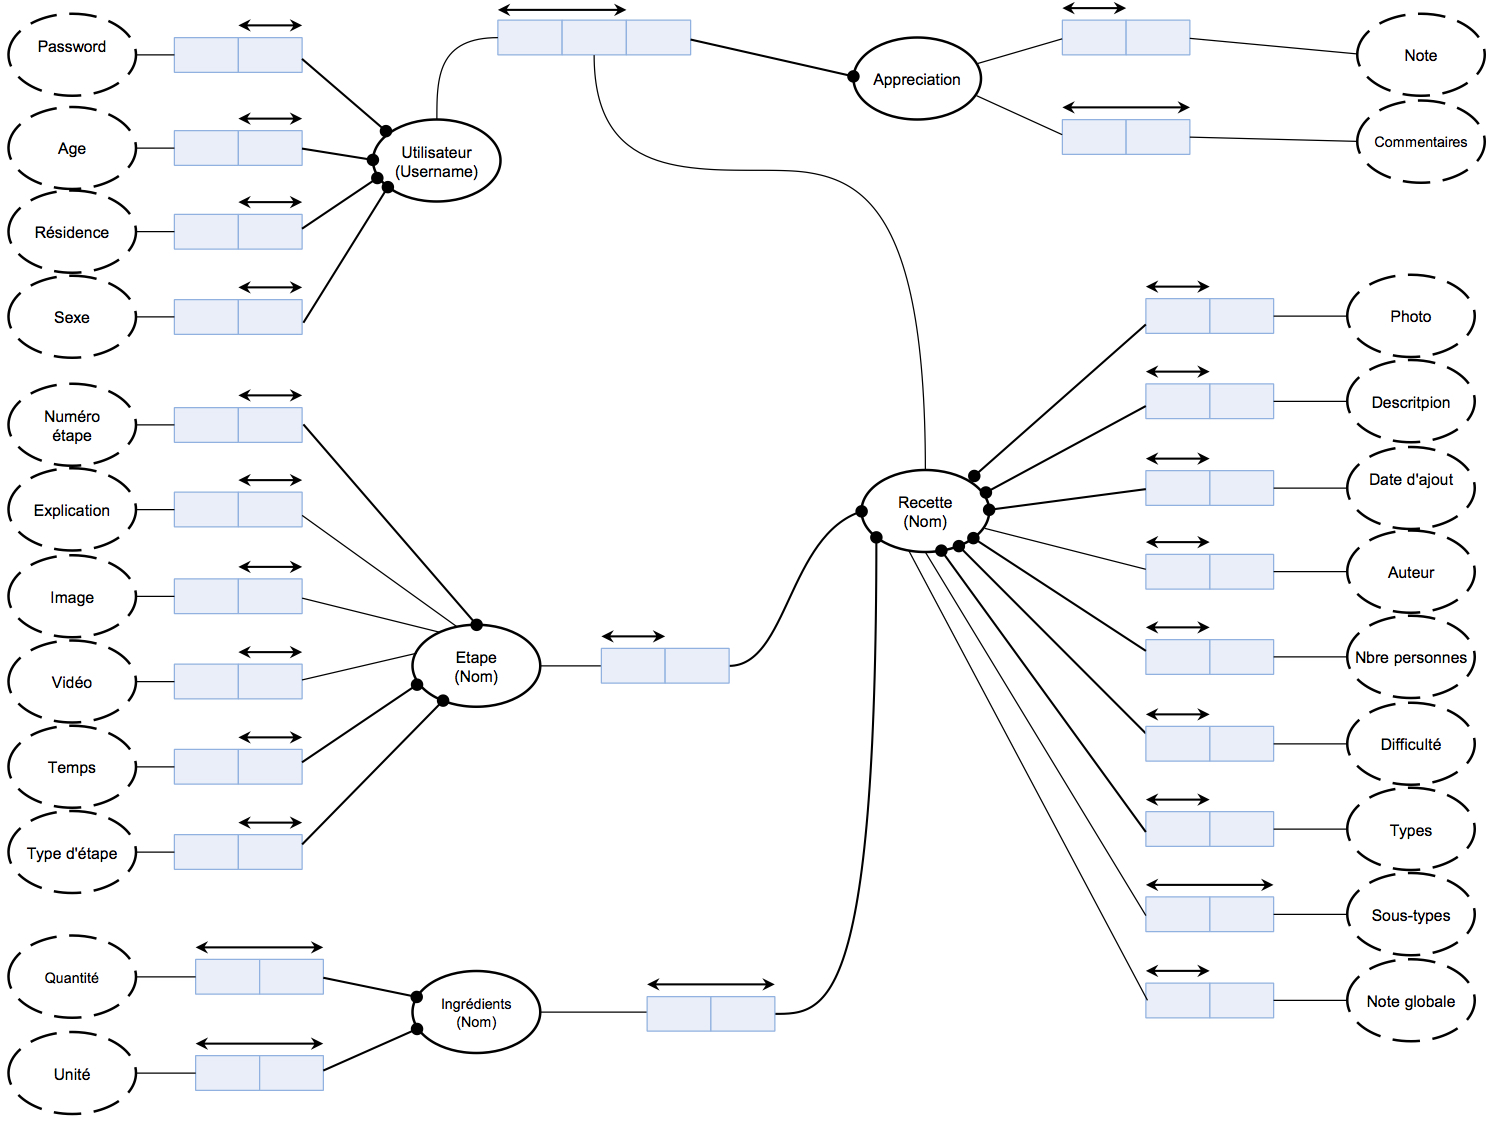
\includegraphics[scale = 0.2]{SchemaORM.jpg}
	\caption{Schema ORM de l'application EZMeal}
	\label{ORM}
\end{figure}

\pagebreak

\chapter{Conception et contenu des differents tableaux}

La base de donnees et l'application sont organisees autour de cinq tableaux differents (Utilisateurs, Recette, Appreciation, Etape et Ingredients), regroupant chacun un nombre variable de champs.  La base de donnees est construite de telle sorte a ce qu'il y ait un maximum de relations binaires et le moins de relations ternaires.

\section{Utilisateurs}

Ce tableau est un element principal de cette application car il stocke les donnees personnelles et interactions sur l'application en memoire. Ce tableau presente un leger inconvenient. En effet, il existe une relation ternaire entre ce tableau et les tableaux recette et appreciation.

Le tableau contient les champs suivants:
\begin{itemize}
	\item Username, ce champ est le champ principal du tableau. Nous l'avons choisi comme tel car nous trouvons que c'est la maniere la plus adequate de qualifier un utilisateur. Ce champ est unique pour un utilisateur car c'est ce qui caracterise un utilisateur.
	\item Password, ce champ est obligatoire et unique pour un utilisateur donne. pour des raisons de securite.
	\item Age, ce champ est obligatoire et unique pour un utilisateur. Ces deux conditions sur la relation sont specifiees dans le canevas de l'application.
	\item Residence, ce champ est obligatoire et unique pour un utilisateur. Ces deux conditions sur la relation sont specifiees dans le canevas de l'application.
	\item Sexe, ce champ est obligatoire et unique pour un utilisateur. Ces deux conditions sur la relation sont specifiees dans le canevas de l'application.
	\item Appreciation, ce champ n'est pas unique et obligatoire pour un utilisateur car nous pensons que, meme si il est utile pour les autres utilisateur d'avoir un avis sur une recette, tous les utilisateurs ne sont pas obliges de donner une appreciation.
	\item Recette, ce champ n'est pas unique et obligatoire car nous pensons que c'est a chacun de decider s'il veut creer une recette ou non.
\end{itemize}

\section{Appreciation}

Ce tableau n'est pas l'extension qui nous devons implementer. C'est un choix purement subjectif d'extension supplementaire a faire car nous nous sommes dits que ce serait mieux pour l'experience utilisateur de pouvoir communiquer sur les recettes, emettre son avis et des conseils/ajustements sur la recette. Le principal desinconvenient de ce tableau est le fait qu'il y ait une relation ternaire entre ce tableau et les tableaux recette et utilisateur.

Le tableau contient les champs suivants:
\begin{itemize}
	\item Username, ce champ n'est pas obligatoire et pas unique car les utilisateurs ne sont pas obliges de donner une appreciation
	\item Note, ce champ n'est pas obligatoire mais est unique pour une appreciation car nous pensons que, pour une appreciation, il n'est pas obligatoire de donner une note mais chaque appreciation ne peut contenir qu'une seule note.
	\item Commentaires, ce champ n'est pas obligatoire et n'est pas unique car une appreciation peut contenir plusieurs commentaires mais n'est pas obligatoirement rempli.
\end{itemize}

\section{Recette}

Ce tableau est l'element principal de l'application. En effet, ce tableau est connecte a tous les autres tableaux et l'application est principalement base sur cette base de donnees. Cependant, ce tableau a une relation ternaire avec les tableaux utilisateur et appreciation.

\end{document}
